%!TEX root = ../Thesis.tex

%
% Add more algorithms from this paper and argue why you've choosen certain algo: multiple_path_planning_algos 
%
Grid-based path-planning algorithms are commonly used in single-agent path planning scenarios. Those algorithms are usually based on graphs and represent a map as a set of vertices and edges. The graph can be either undirected or directed, depending on whether the agent is allowed to move in both or in just one direction between vertices \cite{basic_algorithms}. Only three algorithms will be discussed in this section: Dijkstra's Algorithm, A* Algorithm, and BFS algorithm, as they are useful for further understanding of more complex algorithms. A diagram explaining the general approach for graph-based path planning is shown in figure \ref{fig:simple_path_planning}. 



It is assumed that the grid map of the environment has been translated into a graph representation, with each cell of the grid map being represented by a node in the graph. The starting point and the goal of the robot's path are also known and provided as input to the algorithm.

The execution of the algorithm begins by initializing the starting node as the current node and adding its neighboring nodes to the frontier. The frontier is usually represented by a data structure such as a priority queue, where the priority of each node is determined by algorithm-specific conditions such as the distance from the starting point, the distance to the goal, or a combination of both. At each iteration, the algorithm selects the node with the highest priority from the frontier and expands it by adding its neighboring nodes to the frontier. The algorithm then calculates a condition for each neighboring node. Once a node is expanded, the algorithm checks if the node is the goal node. If this is the case, the algorithm terminates and the path from the starting point to the goal is returned. If the node is not the goal node, the algorithm continues by selecting the next node from the frontier and repeating the process. If at any point the frontier becomes empty, this indicates that there is no route from the starting point to the goal, and the algorithm terminates without finding a path \cite{multiple_path_planning_algos}.
\begin{figure}[H]
    \centering
    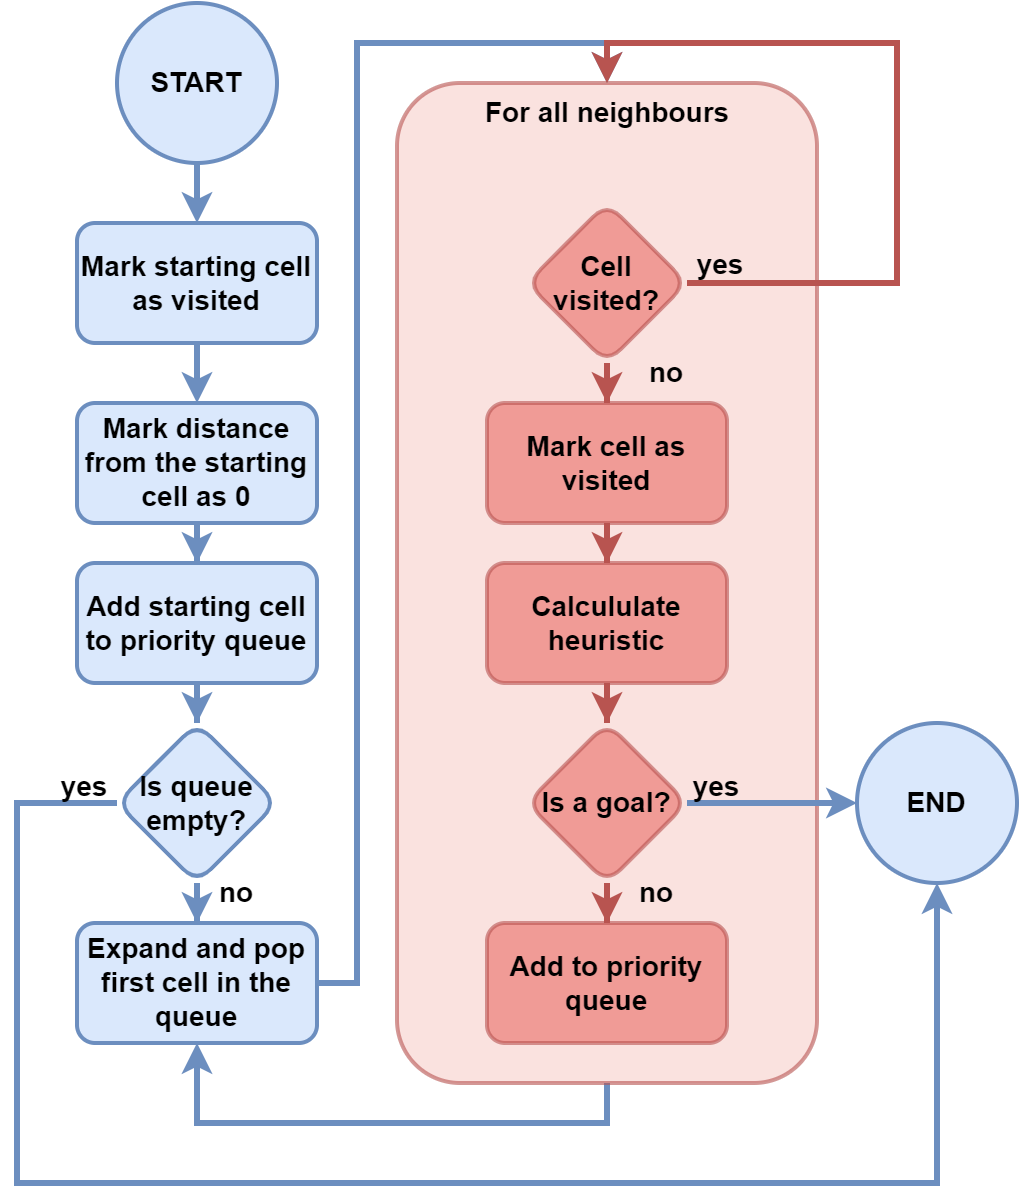
\includegraphics[width=0.7\textwidth]{pictures/simple_algos.png}
    \caption{General approach for graph-based path planning algorithms}
    \label{fig:simple_path_planning}
\end{figure}
\subsection{Dijkstra's Algorithm}
Dijkstra's algorithm is a graph traversal technique that assigns a minimal length, represented by the edge value g(n), from a designated starting vertex to every vertex in a graph. The starting vertex is initially assigned a length of 0, while all other vertices are assigned a length of infinity. The algorithm proceeds by iteratively expanding new vertices, specifically those that are neighbours of the vertex with the current lowest length from the starting vertex, and marking them as visited. The process continues until all vertices have been visited or the goal vertex is reached. If the goal is not reached, the expansion process continues. The algorithm is guaranteed to find the shortest path from the starting vertex to the goal, as long as all edges have non-negative weights \cite{basic_algorithms, basic_2}.

\subsection{Greedy Best-First-Search}
This algorithm is a variant of graph traversal that employs a heuristic function - denoted as h(n), to guide the exploration of vertices. Heuristic function is a formula to determine the cost of reaching a goal. Rather than prioritizing the vertices with the shortest distance from the starting vertex, as in Dijkstra's algorithm, this algorithm prioritizes vertices that are estimated to be closest to the goal vertex using the heuristic function h(n) 
  \cite{a_star_dijkstra}. This approach is referred to as a greedy strategy, as it prioritizes reaching the goal as quickly as possible, without taking into account potential obstacles. The algorithm is fast in terms of computational complexity, but the paths it finds are often sub-optimal.

\subsection{A* Algorithm}
A*(pronounced A star) is the most popular choice for pathfinding, because of its simplicity and robustness. It has also many advanced extensions used in a multi-agent systems approach. It works very similarly to Dijkstra's algorithm, except it is also using heuristics to guide itself. It combines the information about the distance from the start - \(g(n)\) and the heuristic function which is usually a distance to a goal - \(h(n)\). In each iteration, it examines the node that has the lowest sum of \(g(n) + h(n)\) \cite{basic_2}.

The behavior of A* algorithm will vary, depending on the heuristic function that is being used. It is usually faster than Dijkstra when finding a solution, but a result can be sub-optimal so it is a challenge to balance those two.
